\documentclass[conference]{IEEEtran}
\IEEEoverridecommandlockouts
\usepackage{cite}
\usepackage{amsmath,amssymb,amsfonts}
\usepackage{graphicx}
\usepackage{textcomp}
\usepackage{xcolor}
\usepackage{booktabs}
\usepackage{array}
\usepackage{multirow}
\usepackage{url}
\graphicspath{{../results/}}
\newcolumntype{L}[1]{>{\raggedright\arraybackslash}p{#1}}

\begin{document}

\title{Telecom Customer Churn Timing Analysis Using Machine Learning:\\A Comparative Study of Survival Models}

\newcommand{\authorcell}[4]{%
  \begin{tabular}[t]{c}
    \large #1\\[0.2ex]
    \small #2\\
    \small #3\\
    \small #4\\
    \small Bengaluru
  \end{tabular}}

\newcommand{\authorgrid}{%
  \begin{tabular}{@{}c@{\hspace{0.25in}}c@{\hspace{0.25in}}c@{}}
    \authorcell{Sahil Singh}{ENG23CS0435}{eng23cs0435@dsu.edu.in}{Dayananda Sagar University,} &
    \begin{tabular}[t]{c}
    \large Prof. Surajit Sahoo\\[0.2ex]
    \small Project Guide\\
    \small surajit-cse@dsu.edu.in\\
    \small Assistant Professor\\
    \small Dayananda Sagar University,\\
    \small Bengaluru
  \end{tabular} &
    \authorcell{Sachkirat Singh Arora}{ENG23CS0434}{eng23cs0434@dsu.edu.in}{Dayananda Sagar University,} \\
    \rule{0pt}{5ex}\authorcell{Samarth BS}{ENG23CS0438}{eng23cs0438@dsu.edu.in}{Dayananda Sagar University,} &
    \relax &
    \rule{0pt}{5ex}\authorcell{Sattwik Khan}{ENG23CS0444}{eng23cs0444@dsu.edu.in}{Dayananda Sagar University,} \\
  \end{tabular}}

\author{\authorgrid}

\maketitle

\begin{abstract}
Most churn studies on telecom data ask who will leave. Survival studies on the same data go one step further and ask how long customers stay, but they still report one number per attribute, as if price, payment method or internet type mattered the same in the first month and in the third year. This paper asks a narrower question: in which part of tenure does a known risk factor actually act? We turn 7,032 customers of the public IBM Telco sample into one row per month and model the chance of leaving in a given month with logistic regression. A search looks at 57 candidates. Each candidate is an attribute paired with one of three tenure windows (month 1, months 2--6, months 7--24), and it is kept only when adding it clearly improves the fit, after a correction for the number of candidates tried. The search runs on one half of the customers. The other half, which the search never sees, is used to estimate the selected terms and to score predictions. The whole procedure is repeated over five random splits. Monthly charge in month 1 was selected in all five splits, and monthly charge in months 2--6 and fiber optic in month 1 in four. On the held-out halves the selected terms were jointly significant every time ($p < 3\times10^{-11}$). Holding the service bundle fixed, a one-standard-deviation higher monthly charge cut the odds of leaving in month 1 to 0.24 times the later-tenure effect (95\% CI 0.16--0.37). The screened model lowered the month-1 Brier score by 3.4\% and a window-specific calibration error by 20--23\% against a level-effect model and a Cox model. It matched a gradient-boosted model on early-tenure accuracy and had the best overall Brier score of the four models in all five splits. A ranking score, Harrell's C-index, barely moved (about 0.86 for every model), which shows that ordering customers correctly is not the same as placing their risk in the right month. A contract-renewal window, the usual timing story in telecom, was checked separately and showed no effect (odds ratio 1.02, 95\% CI 0.37--2.77).
\end{abstract}

\begin{IEEEkeywords}
Customer churn, machine learning, survival analysis, discrete-time hazard, model comparison, telecommunications
\end{IEEEkeywords}

\section{Introduction}

Customer churn is one of the oldest problems in applied analytics. A small rise in retention can have a large effect on profit, and telecom operators have long built models to flag customers who are about to leave. Nearly all of this work treats churn as a yes-or-no label attached to each customer. Logistic regression, random forests, boosted trees and neural networks are trained on that label and compared on accuracy or area under the ROC curve. The label hides an important fact: a customer who is still active has not proven loyal. That customer has simply not been observed long enough. Treating such a customer as a negative case mixes up two different things, staying and not yet having left.

Survival analysis removes this confusion by treating tenure as the clock and active customers as censored observations \cite{cox1972}. On the IBM Telco sample, which is now the standard public benchmark for churn, survival models have been fitted many times. Kaplan--Meier curves, Cox regression and parametric models all agree that month-to-month contracts, payment by check, fiber-optic service and the absence of add-on services such as online security raise the hazard of leaving \cite{rahman2024,ishtiaq2026,havrylovych2019}. These are useful findings, but they share a hidden assumption. A Cox model reports one hazard ratio per attribute, which means an attribute is assumed to have the same relative effect in month 1 as in month 40. When that assumption fails, published studies usually stratify the offending variable away or drop it \cite{ishtiaq2026,masarifoglu2019}. Neither choice says where in tenure the effect is concentrated.

For a retention team the location of an effect is not a detail. An effect that is concentrated in the first month calls for onboarding action at sign-up. An effect that is spread over years calls for a loyalty program. Two models with the same C-index can send a manager to very different places. The question this paper asks is therefore not ``who leaves'' or ``how long do they stay'' but ``in which part of tenure does each risk factor act, and can that be shown without fooling ourselves?''

The last part of the question matters. If one looks at hazard plots, picks the windows that look unusual and then tests them on the same data, the resulting p-values are meaningless. We handle this with a screen-then-confirm design based on sample splitting \cite{cox1975}. The contributions of this paper are:

\begin{itemize}
\item A screen-then-confirm protocol for monthly churn risk. A search over attribute-by-tenure-window effects runs on a discovery half. Estimation, tests and prediction scores use only a confirmation half. Repeating this over several splits shows how often each term is picked.
\item A window calibration error that measures how far a model's predicted exits fall from the exits actually seen, inside fixed customer groups and tenure windows. Unlike the C-index, it penalises a model that ranks customers correctly but places their risk in the wrong month.
\item Evidence on the IBM Telco sample that the most stable tenure-localised effect is monthly price in the first month, that this effect is missed by a global proportional-hazards test, and that the popular contract-renewal timing hypothesis does not hold in these records.
\item A three-term interpretable hazard model that matches a gradient-boosted hazard on early-tenure accuracy and beats it on integrated Brier score, with a fully reproducible open pipeline.
\end{itemize}

\section{Literature Review}

The related literature is summarised in Table~\ref{tab:related}.

Most published churn work treats the problem as classification. Each customer gets a yes-or-no label, and models such as logistic regression, random forests and boosted trees are compared on accuracy. That setup does not use tenure. A customer who is still with the company is coded the same way as a customer who has been loyal for years.

Survival models put time back in. On the IBM Telco sample, Rahman et al. \cite{rahman2024} combined Kaplan--Meier estimates, a stratified Cox model and a Fine--Gray competing-risk model, and reported a concordance of 0.867. Havrylovych and Kuznietsova \cite{havrylovych2019} compared Cox, Weibull and log-normal models on the same data and gave rules for forecasting the period in which a customer's risk starts to rise. Ishtiaq \cite{ishtiaq2026} combined Cox regression with three classifiers and a cost analysis, and found that the proportional-hazards assumption failed for contract type. The fix used there was a contract-stratified model, which sets the problem aside rather than saying in which month the effect acts. Fernandez et al. \cite{fernandez2024} compared Cox, accelerated failure time, random survival forest, DeepSurv and ensembles on several datasets, including IBM Telco. On this sample the Cox model was hard to beat on both the C-index and the integrated Brier score.

A single hazard ratio is often a poor description of telecom churn. Masarifoglu and B\"uy\"ukl\"u \cite{masarifoglu2019} tested the proportional-hazards assumption with Schoenfeld residuals \cite{grambsch1994} on operator data and dropped the variable that failed the test. Shapoval and Setzer \cite{shapoval2015} argued that fixed-term contracts should produce extra cancellations near the contract end, and showed that features built from real contract dates improved prediction on operator data. These studies show that timing matters. Each one either drops the awkward variable or fixes the time pattern in advance.

The gap is straightforward. Survival studies of telecom churn estimate how strongly an attribute raises risk, not in which part of tenure it does so. None of the studies above chooses tenure-specific terms on one half of the customers and tests them on the other half. None of them checks whether a model places the risk in the right month, rather than only ranking the right customers. This paper does both, and then compares the resulting model with a level-effect hazard, a Cox model and a gradient-boosted hazard.

\begin{table*}[t]
\caption{Summary of related work on survival-based churn analysis}
\label{tab:related}
\centering
\footnotesize
\begin{tabular}{L{2.5cm}L{2.5cm}L{3.7cm}L{3.4cm}L{3.7cm}}
\toprule
Author & Method & Contribution & Advantages & Limitations \\
\midrule
Rahman et al. (2024) \cite{rahman2024} & KM, stratified Cox, Fine--Gray & Competing-risk survival analysis of IBM Telco & Separates two exit causes; concordance 0.867 & One hazard ratio per attribute; no hold-out test \\
Ishtiaq (2026) \cite{ishtiaq2026} & KM, Cox, LR, RF, GBM & Joint survival and classifier study with cost analysis & Hold-out calibration; reports PH failure for contract & Contract stratified away; timing of effects not examined \\
Havrylovych and Kuznietsova (2019) \cite{havrylovych2019} & Cox, Weibull, log-normal & Forecast of the period when churn risk rises & Gives segment-level timing of risk & Same parametric time shape for every attribute \\
Masarifoglu and B\"uy\"ukl\"u (2019) \cite{masarifoglu2019} & Extended Cox, Schoenfeld tests & Time-dependent campaign covariate in operator data & Formal PH testing & Violating covariate dropped rather than modelled \\
Fernandez et al. (2024) \cite{fernandez2024} & Cox, AFT, RSF, DeepSurv, ensembles & Benchmark across three datasets incl. Telco & Cox strongest on Telco by C-index and IBS & Ranking and global error only \\
Shapoval and Setzer (2015) \cite{shapoval2015} & Cox with contract-date features & Contract-end timing in churn & Better out-of-sample prediction & Needs contract dates; proprietary data \\
This work & Discrete hazard, four-model comparison & Locates and confirms tenure-specific churn effects & Split-sample test; window calibration & Single public sample; associational \\
\bottomrule
\end{tabular}
\end{table*}

\section{Dataset Description}

The study uses the IBM Telco Customer Churn sample \cite{ibmtelco}, a public file that describes 7,043 customers of a fictional telecom provider. Each row is one customer. The file records demographics (gender, senior-citizen status, partner, dependents), the account (tenure in months, contract type, paperless billing, payment method, monthly and total charges) and services (phone, multiple lines, internet type, online security, online backup, device protection, technical support, streaming TV and streaming movies). The outcome column, \textit{Churn}, says whether the customer left within the last month of the observation window.

Eleven customers have a blank total charge and a tenure of zero, so they were removed, leaving 7,032 customers. Of these, 1,869 (26.6\%) left and 5,163 (73.4\%) were still active and are treated as right-censored at their recorded tenure. Tenure runs from 1 to 72 months. The first month is unusual: 613 customers have a tenure of one month, and 380 of them left, which is 20\% of all exits in the file. Contract type separates customers sharply. Month-to-month customers left at a rate of 42.7\%, one-year customers at 11.3\% and two-year customers at 2.8\%, and no one-year or two-year customer left in month 1.

Total charges were not used as a covariate because they are, apart from price changes, the product of tenure and monthly charge, and tenure is the outcome clock. Monthly charge was standardised with the mean and standard deviation of the discovery half in each split. Every other attribute was coded as a 0/1 indicator. Online security, online backup, device protection and technical support were coded as an explicit ``No'', so that customers without internet are not counted as lacking the add-on; an indicator for no internet service carries that information instead. Payment method was coded with bank transfer as the reference. This gives 21 standing attributes, listed in Table~\ref{tab:ph}.

\section{Proposed Methodology}

Fig.~\ref{fig:pipeline} shows the pipeline. Each step is described below.

\begin{figure*}[t]
\centering
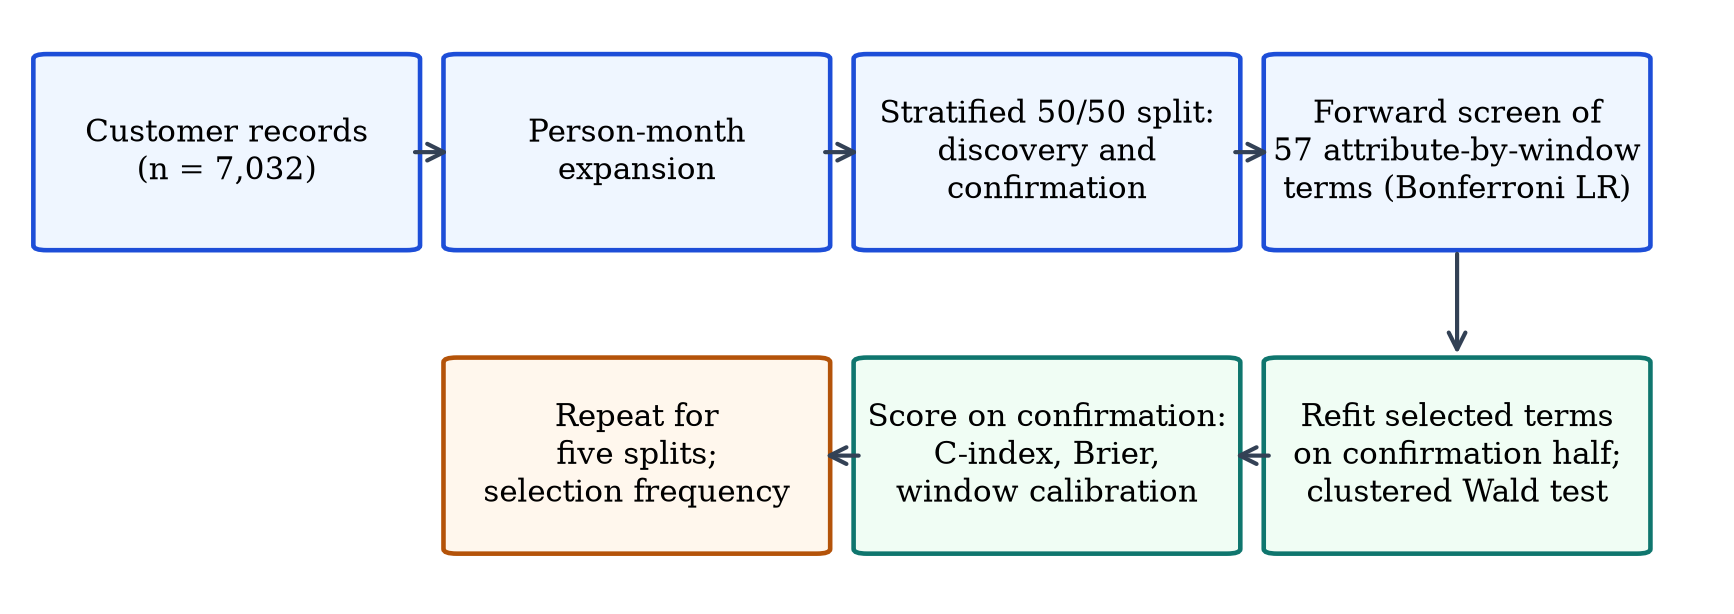
\includegraphics[width=0.86\textwidth]{fig_pipeline.png}
\caption{Screen-then-confirm pipeline. The discovery half chooses the terms; the confirmation half, never seen by the screen, estimates them, tests them and scores the models. The procedure is repeated for five random splits.}
\label{fig:pipeline}
\end{figure*}

\subsection{Person-Month Representation}

Tenure is stored in whole months, so we work month by month. Write $T_i$ for the last month we see customer $i$, and let $\delta_i = 1$ if the customer left in that month and $0$ if they were still active. The quantity we model is the chance of leaving in month $t$, given that the customer was still active at the start of it:
\begin{equation}
h_i(t) = \Pr(T_i = t \mid T_i \ge t, \mathbf{x}_i),
\end{equation}
where $\mathbf{x}_i$ is the customer's attributes. Each customer becomes one row per month at risk, from month 1 up to $T_i$. That row is marked as an exit only when the customer actually left in that month. Logistic regression on these rows estimates $h_i(t)$ \cite{allison1982}. The chance of still being active after several months is the product of the chances of not leaving in each of those months. Each discovery half produced about 114,000 person-month rows.

\subsection{Level-Effect Hazard Model}

The reference model lets each attribute shift the chance of leaving by the same amount in every month:
\begin{equation}
\operatorname{logit} h_i(t) = \alpha(t) + \boldsymbol{\beta}^{\top}\mathbf{x}_i .
\end{equation}
The logit is the log-odds, $\log\bigl(h/(1-h)\bigr)$. The baseline $\alpha(t)$ is the shared risk in month $t$. It has to be flexible. If it is too stiff, an early-window term can look important only because it is patching a poor fit for the first few months. Months 1, 2 and 3 therefore get their own intercepts, and the baseline also includes $\log t$, tenure in years, and the square of tenure in years. This is the ``level'' model in the comparisons below. It has no tenure-specific terms: a factor that matters in month 1 is forced to matter in the same way in month 40.

\subsection{Tenure-Window Terms}

Three windows were fixed before any search was run. Month 1 is the first, months 2--6 the second, and months 7--24 the third. Months after 24 are the comparison period. A candidate is one attribute switched on only inside one window. Its coefficient says how much that attribute's effect changes inside the window, relative to later months.

Contract type stays a level effect only. One-year and two-year customers have no exits in month 1, so a contract-by-window term cannot be estimated. The other 19 attributes and three windows give 57 candidates. If $\mathcal{S}$ is the set of pairs the screen keeps, the screened model is the level model plus one extra coefficient for each pair:
\begin{equation}
\operatorname{logit} h_i(t) = \alpha(t) + \boldsymbol{\beta}^{\top}\mathbf{x}_i + \sum_{(j,w)\in\mathcal{S}} \gamma_{jw}\, x_{ij}\,\mathbf{1}[t \in W_w].
\end{equation}
The indicator $\mathbf{1}[t \in W_w]$ is 1 only in the months of window $w$, so $\gamma_{jw}$ does not touch the rest of tenure.

\subsection{Forward Screen on the Discovery Half}

Customers were split in half at random, with the same share of leavers in each half. On the discovery half the search starts from the level model. At each step it refits once for every candidate still in the pool and keeps the one that improves the fit the most, but only if that improvement is unlikely to be chance. The bar is $0.05$ divided by the number of candidates still waiting, which is the Bonferroni correction. The first term has to beat $0.05/57 \approx 0.0009$. The search stops when the next candidate fails this bar, or after eight terms, whichever comes first.

\subsection{Confirmation on the Held-Out Half}

The selected set is then frozen. On the confirmation half the level model and the screened model are fitted again from scratch, and the selected terms are tested together against the level model. Two tests are reported: a likelihood-ratio test, which asks whether the extra terms improve the fit, and a Wald test, which asks whether their coefficients are jointly different from zero. Rows from the same customer are not independent, so the Wald test and the confidence intervals use standard errors clustered by customer. The confirmation customers took no part in choosing the terms, so these tests mean what they usually mean \cite{cox1975}.

\subsection{Benchmark Models}

Three benchmarks are fitted on the discovery half and scored on the confirmation half, in the same way as the screened model:
\begin{itemize}
\item \textbf{Level hazard:} equation (2), with no window terms.
\item \textbf{Cox model} \cite{cox1972}: the standard survival model with the same 21 attributes, fitted with the lifelines library. It also forces each attribute to have one effect for the whole of tenure. Monthly chances of leaving were read off its predicted survival curve.
\item \textbf{Boosted hazard:} a gradient-boosting classifier trained on the person-month rows, with the 21 attributes and the month number as inputs. Unlike the other models it is not told which windows to use, so it can pick up any pattern between attributes and tenure. It used up to 400 trees, a learning rate of 0.05, at most 15 leaves per tree, at least 200 rows per leaf, an L2 penalty of 1, and early stopping on a 15\% validation slice.
\end{itemize}

\subsection{How the Models Are Scored}

All scores use the confirmation half only, and are averaged over five splits (random seeds 42, 7, 19, 101 and 2024).

\textit{Ranking.} Harrell's C-index checks whether a customer who left sooner was given a lower chance of still being active at month 24. It only looks at the order of customers. Moving one customer's risk from month 6 to month 1 barely changes it.

\textit{Accuracy over time.} The Brier score measures how far predicted chances sit from what happened, with a weight that corrects for customers who are still active \cite{graf1999}. It is reported at months 1, 3, 6, 12 and 24. The integrated Brier score is the average from month 1 to month 24. Lower is better.

\textit{Window calibration.} For a customer group $g$ and a tenure window $w$, let $O_{gw}$ be the exits observed, $E_{gw}$ the exits the model expected, and $N_{gw}$ the number of customer-months at risk. The window calibration error is the average gap per customer-month:
\begin{equation}
\mathrm{WCE}_w = \frac{\sum_g \lvert O_{gw} - E_{gw}\rvert}{\sum_g N_{gw}}.
\end{equation}
The groups are the twelve combinations of payment method and internet type. They were fixed before scoring and are the same for every model, so the grouping does not favour one model.

\textit{Negative control.} On the primary split the screened model was fitted again on the confirmation half with one extra term, equal to one for one-year contracts in months 11--13 and for two-year contracts in months 23--25. If people leave when a contract comes up for renewal, this term should be large.

\subsection{Constant-Effect Check}

For comparison with earlier papers, a Cox model with all 21 attributes was fitted on the full sample. Each attribute was then checked to see whether its effect stays constant over tenure, using the scaled Schoenfeld residual test with rank time \cite{grambsch1994}. A pass on this test is often read as ``the effect does not change with tenure.'' The screen below is a more direct check of that reading.

\section{System Modules}

\subsection{Data Processing Module}
This module reads the raw file, removes the eleven records with blank total charges, converts tenure to the event clock and the churn flag to the event indicator, and codes every attribute as described in Section~III.

\subsection{Person-Month Expansion Module}
This module converts each customer into one row per month at risk and attaches the event indicator for the final month. It also builds prediction panels in which every confirmation customer is followed for 24 months.

\subsection{Screening Module}
This module runs the forward likelihood-ratio search on the discovery half, logs every step with its statistic and threshold, and returns the frozen set of window terms.

\subsection{Confirmation Module}
This module refits the selected model on the confirmation half, computes customer-level standard errors, the joint tests of the selected terms, and the renewal-window check.

\subsection{Evaluation Module}
This module fits the benchmarks, turns every model into a monthly chance of leaving, and computes the C-index, Brier scores and window calibration error. It repeats the process across splits and records how often each term is selected.

The pipeline is written in Python with statsmodels, lifelines and scikit-learn. A full run takes about one minute on a laptop.

\section{Results and Analysis}

\subsection{What the Raw Hazards Show}

Fig.~\ref{fig:empirical} plots monthly exit hazards for the full sample. These plots are descriptive and played no part in the screen. Panel (a) splits customers into quartiles of monthly charge. In month 1 the middle quartiles lose 8.1\% and 7.1\% of their customers, the lowest quartile 5.0\%, and the highest quartile only 1.5\%. From month 7 to month 24 the ordering changes: the highest quartile then leaves at 0.66\% a month, more than the lowest quartile at 0.22\%. Panel (b) shows the familiar gap by payment method. The gap is widest in month 1, when 8.8\% of check payers leave against 1.0\% of automatic payers.

\begin{figure*}[t]
\centering
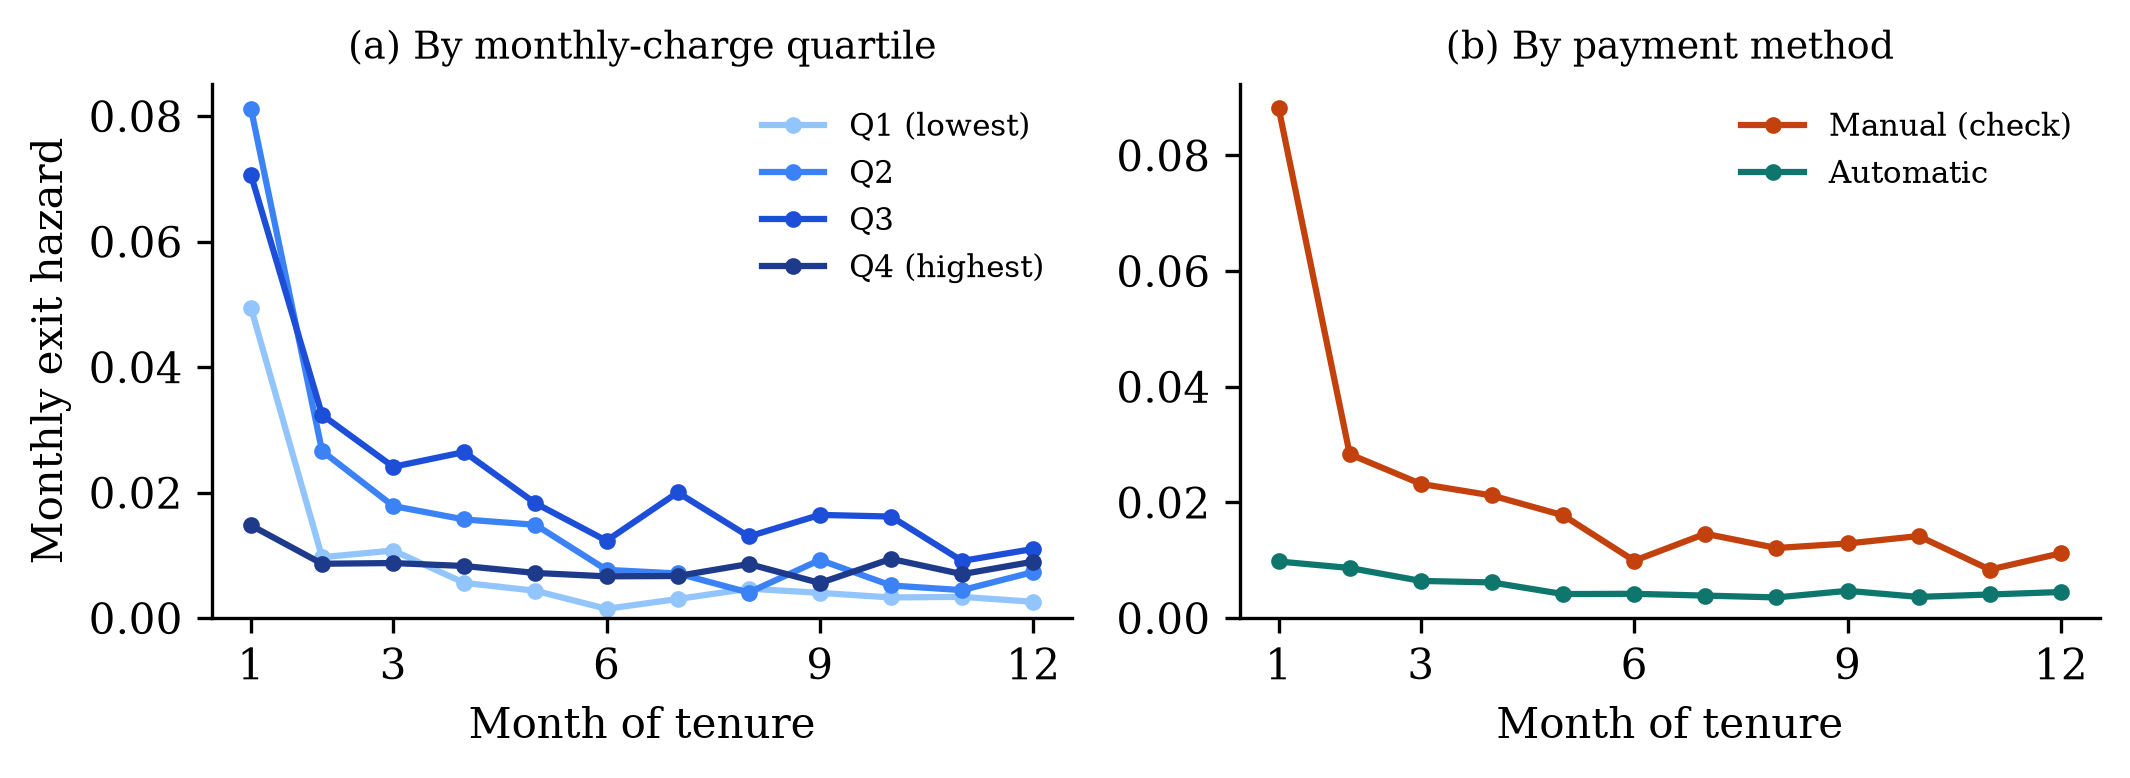
\includegraphics[width=0.82\textwidth]{fig_empirical.png}
\caption{Observed monthly exit hazard over the first year, all 7,032 customers. (a) By quartile of monthly charge. (b) Manual (electronic or mailed check) versus automatic payment.}
\label{fig:empirical}
\end{figure*}

\subsection{The Global Proportional-Hazards Test}

Table~\ref{tab:ph} lists the Schoenfeld test for each attribute in the full-sample Cox model. As earlier studies found \cite{ishtiaq2026}, both contract indicators fail clearly. Several add-on services and both check payment methods also fail at the 5\% level. Monthly charge does not ($p = 0.25$), and neither does fiber optic ($p = 0.17$). A reader relying on this test would conclude that the effect of price is constant over tenure. The screen below shows that this conclusion is wrong, because a test that averages over all event times can miss an effect concentrated in one short window.

\begin{table}[t]
\caption{Schoenfeld test of proportional hazards, full-sample Cox model (rank time)}
\label{tab:ph}
\centering
\footnotesize
\begin{tabular}{lrrr}
\toprule
Attribute & HR & $\chi^2_1$ & $p$ \\
\midrule
One-year contract & 0.199 & 39.61 & $<$0.001 \\
Two-year contract & 0.040 & 16.71 & $<$0.001 \\
Mailed check & 1.761 & 8.82 & 0.003 \\
Multiple lines & 0.658 & 7.91 & 0.005 \\
No tech support & 1.447 & 7.88 & 0.005 \\
No online security & 1.844 & 7.81 & 0.005 \\
No online backup & 1.846 & 4.67 & 0.031 \\
Electronic check & 1.797 & 4.64 & 0.031 \\
Has partner & 0.596 & 4.48 & 0.034 \\
No internet & 1.779 & 4.21 & 0.040 \\
Streaming TV & 1.042 & 3.98 & 0.046 \\
Fiber optic & 1.798 & 1.87 & 0.172 \\
Monthly charge (per SD) & 0.785 & 1.35 & 0.246 \\
\bottomrule
\multicolumn{4}{l}{\scriptsize Eight further attributes have $p > 0.05$ and are omitted.}
\end{tabular}
\end{table}

\subsection{Screening and Confirmation}

On the primary split the screen kept three terms. Monthly charge in month 1 entered first (likelihood-ratio statistic 46.3), fiber optic in month 1 second (30.6) and monthly charge in months 2--6 third (18.5). The next candidate, missing online security in months 2--6, scored 9.6 ($p = 0.0019$) and did not beat the threshold of about 0.0009, so the search stopped.

Table~\ref{tab:freq} shows how often each term was selected across the five splits. Monthly charge in month 1 was chosen every time. Monthly charge in months 2--6 and fiber optic in month 1 were chosen four times each. Six other terms appeared once each and should be read as unstable. On the confirmation halves the selected set was jointly significant in every split, with likelihood-ratio statistics between 58.5 and 79.7 and clustered Wald p-values between $2\times10^{-16}$ and $1.4\times10^{-11}$.

\begin{table}[t]
\caption{Selection frequency over five discovery halves}
\label{tab:freq}
\centering
\footnotesize
\begin{tabular}{lc}
\toprule
Term (attribute $\times$ window) & Splits \\
\midrule
Monthly charge $\times$ month 1 & 5/5 \\
Monthly charge $\times$ months 2--6 & 4/5 \\
Fiber optic $\times$ month 1 & 4/5 \\
Credit card $\times$ month 1 & 1/5 \\
Streaming TV $\times$ months 2--6 & 1/5 \\
Fiber optic $\times$ months 7--24 & 1/5 \\
Phone service $\times$ month 1 & 1/5 \\
No tech support $\times$ month 1 & 1/5 \\
No online security $\times$ months 2--6 & 1/5 \\
\bottomrule
\end{tabular}
\end{table}

Table~\ref{tab:confirm} and Fig.~\ref{fig:forest} give the confirmation estimates for the primary split. An odds ratio below 1 means the attribute is linked to staying, relative to its effect after month 24. One standard deviation of monthly charge (about \$30) brings the odds of leaving in month 1 down to 0.24 times that later effect, and to 0.65 times in months 2--6. Fiber optic moves the other way: in month 1 its odds ratio is 2.94. The two terms should be read together. Fiber plans are the most expensive in the file (mean \$91.5 against \$58.1 for DSL), so the price term alone would say that fiber customers almost never leave in month 1. The fiber term pulls that prediction back toward what is observed. The stable finding is about price. Holding the service bundle fixed, customers who pay more are far less likely to leave in their first month. That association fades over the next five months and is gone by the third year.

\begin{table}[t]
\caption{Selected terms refitted on the confirmation half, primary split (clustered 95\% CI)}
\label{tab:confirm}
\centering
\footnotesize
\begin{tabular}{lccc}
\toprule
Term & OR & 95\% CI & $p$ \\
\midrule
Monthly charge $\times$ month 1 & 0.240 & 0.157--0.367 & $<$0.001 \\
Fiber optic $\times$ month 1 & 2.941 & 1.434--6.035 & 0.003 \\
Monthly charge $\times$ months 2--6 & 0.649 & 0.520--0.809 & $<$0.001 \\
\midrule
\multicolumn{4}{l}{Joint Wald $\chi^2_3 = 68.3$, $p = 1.0\times10^{-14}$; LR $= 67.6$} \\
\bottomrule
\end{tabular}
\end{table}

\begin{figure}[t]
\centering
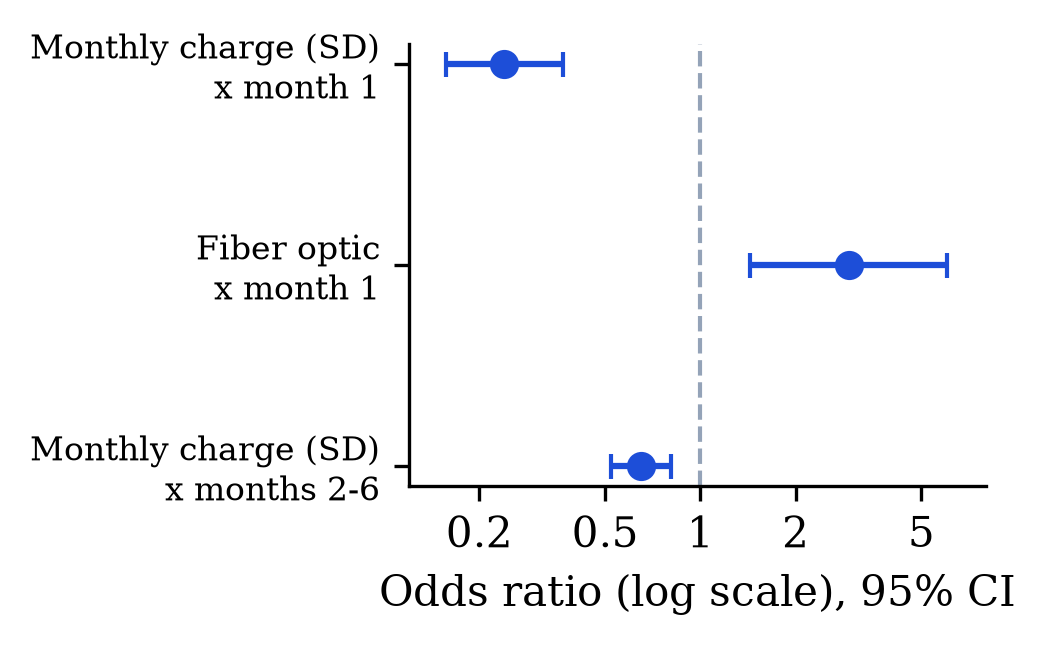
\includegraphics[width=0.95\columnwidth]{fig_forest.png}
\caption{Odds ratios of the selected window terms on the confirmation half of the primary split. Each ratio compares the attribute's effect inside the window with its effect after month 24.}
\label{fig:forest}
\end{figure}

\subsection{Predictive Comparison}

Table~\ref{tab:metrics} reports the hold-out scores. The screened model had the lowest integrated Brier score of the four models (0.0812), and it was lower than every benchmark in all five splits. In month 1 its Brier score was 0.0427 against 0.0442 for both the level and the Cox model, a 3.4\% reduction that held in every split. The gain in window calibration was larger: month-1 WCE fell from 0.0158 (level) and 0.0152 (Cox) to 0.0122, a reduction of 23\% and 20\%. The boosted hazard, which can learn any attribute-by-month pattern, reached the same month-1 accuracy (Brier 0.0427, WCE 0.0120) but had a worse integrated Brier score (0.0820) and the lowest C-index (0.858). The screened model reached the same early accuracy with three extra coefficients that a manager can read off a table.

\begin{table*}[t]
\caption{Hold-out performance on the confirmation halves (mean $\pm$ SD over five splits). Lower is better except C-index.}
\label{tab:metrics}
\centering
\footnotesize
\resizebox{\textwidth}{!}{%
\begin{tabular}{lcccccccc}
\toprule
Model & C-index & IBS (1--24) & Brier@1 & Brier@6 & Brier@12 & Brier@24 & WCE month 1 & WCE all \\
\midrule
Screened hazard (ours) & 0.8625 $\pm$ 0.0033 & \textbf{0.0812} $\pm$ 0.0021 & \textbf{0.0427} $\pm$ 0.0017 & \textbf{0.0742} $\pm$ 0.0030 & \textbf{0.0861} $\pm$ 0.0027 & 0.0925 $\pm$ 0.0017 & 0.0122 $\pm$ 0.0013 & \textbf{0.0020} $\pm$ 0.0003 \\
Level hazard & 0.8633 $\pm$ 0.0029 & 0.0821 $\pm$ 0.0021 & 0.0442 $\pm$ 0.0018 & 0.0763 $\pm$ 0.0028 & 0.0872 $\pm$ 0.0028 & \textbf{0.0915} $\pm$ 0.0018 & 0.0158 $\pm$ 0.0016 & 0.0021 $\pm$ 0.0001 \\
Cox PH & \textbf{0.8635} $\pm$ 0.0030 & 0.0823 $\pm$ 0.0021 & 0.0442 $\pm$ 0.0018 & 0.0765 $\pm$ 0.0030 & 0.0875 $\pm$ 0.0029 & 0.0917 $\pm$ 0.0019 & 0.0152 $\pm$ 0.0014 & 0.0022 $\pm$ 0.0001 \\
Boosted hazard & 0.8584 $\pm$ 0.0025 & 0.0820 $\pm$ 0.0017 & \textbf{0.0427} $\pm$ 0.0016 & 0.0744 $\pm$ 0.0024 & 0.0873 $\pm$ 0.0020 & 0.0935 $\pm$ 0.0017 & \textbf{0.0120} $\pm$ 0.0017 & \textbf{0.0020} $\pm$ 0.0003 \\
\bottomrule
\end{tabular}}
\end{table*}

Fig.~\ref{fig:month1} breaks the month-1 prediction down by payment method on the primary confirmation half. The level model overpredicts month-1 exits among electronic-check payers, whose median charge is \$81, and both the level and Cox models underpredict them among mailed-check payers, whose median charge is \$35 and nearly half of whom have no internet service. Because the screened model lets price act differently in month 1, it moves closer to the observed rate in both groups without any payment-specific term. Credit-card payers are overpredicted by every model, least by the boosted one.

\begin{figure}[t]
\centering
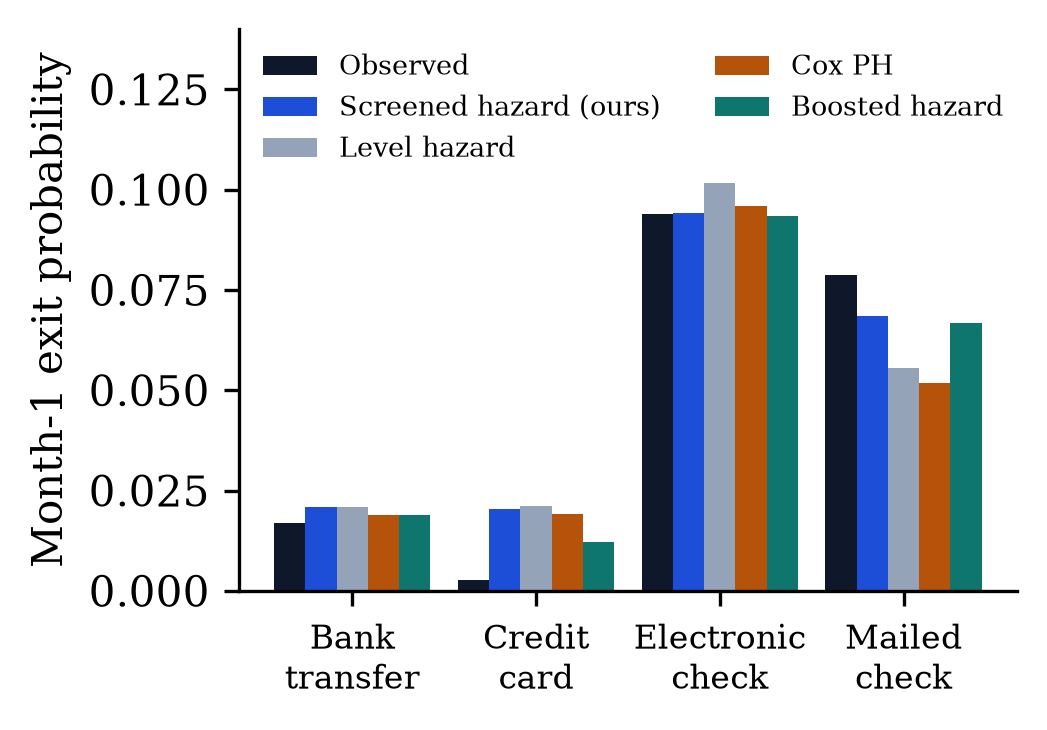
\includegraphics[width=0.95\columnwidth]{fig_month1.png}
\caption{Observed and predicted probability of leaving in month 1 by payment method, confirmation half of the primary split.}
\label{fig:month1}
\end{figure}

Fig.~\ref{fig:brier} shows the Brier score across horizons. From month 1 to month 12 the screened model is either the best or within 0.0001 of the boosted hazard, and it is ahead of the level and Cox models at every one of these horizons. At month 24 the level and Cox models are slightly better (0.0915 and 0.0917 against 0.0925). This is the expected cost of the design: the window terms are built to describe early tenure, and the model gives up a little accuracy far from where its extra terms act.

\begin{figure}[t]
\centering
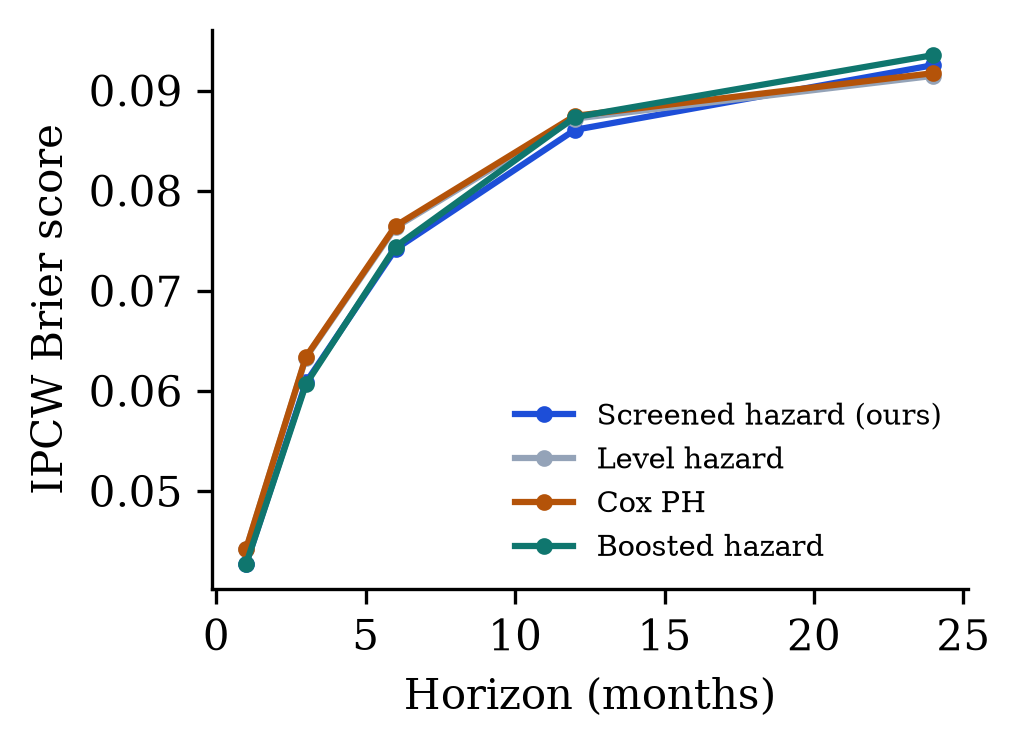
\includegraphics[width=0.95\columnwidth]{fig_brier.png}
\caption{Brier score by horizon, corrected for customers still active. Mean over the five confirmation halves.}
\label{fig:brier}
\end{figure}

The C-index tells a different story from every other measure. All four models sit between 0.858 and 0.864, and the screened model is below the level and Cox models in every split, by 0.0007 and 0.0009 on average. Concordance compares the ordering of customers by predicted survival at a single horizon. Moving risk from month 6 to month 1 for the same customer barely changes that ordering, so the C-index cannot reward a model for putting risk in the right month. Studies that rank churn models only by concordance or AUC will miss this kind of improvement.

\subsection{Negative Control: Contract Renewal}

The renewal-window term had an odds ratio of 1.02 (95\% CI 0.37--2.77, $p = 0.98$). In these records customers on one-year and two-year contracts are no more likely to leave in the months around their renewal date than at other times. The contract-end timing that Shapoval and Setzer \cite{shapoval2015} found in operator data with real contract dates does not appear in the IBM sample, where the only timing information is tenure.

\subsection{Discussion}

Three points deserve comment.

First, the main finding concerns timing, not strength. Price is not new as a churn factor, but treating it as a constant hazard ratio hides the fact that its association with exit changes sign over tenure. A high price is linked to staying in month 1 and, if anything, to leaving later. One reading is that customers who sign up for an expensive bundle have already made a considered choice, while customers on cheap plans are more often trying the service. The data cannot tell these stories apart, but each one points to a different onboarding policy, and neither is visible in a single hazard ratio.

Second, the result depends on how candidates are coded, and we report a sensitivity check that was not part of the planned analysis. In an earlier exploratory look at the same file we had noticed that manual payers leave much more often in month 1 (Fig.~\ref{fig:empirical}b). The screen codes electronic and mailed checks as separate attributes, and neither entered the model. When a pooled ``manual payment $\times$ month 1'' term was added after the screen had finished, it still improved the fit on the primary discovery half (likelihood-ratio statistic 16.6). The pooled term was not in the pre-specified candidate set, so it is a hypothesis for a new sample, not a finding of this paper. The point for practice is that candidate coding should be decided before the data are inspected.

Third, the protocol is general. Nothing in it is specific to telecom or to this dataset. Any subscription business with tenure data can run the same screen, and the WCE can be computed for any model that produces monthly hazards, including black-box models.

\subsection{Limitations}

The IBM Telco file is a vendor-published fictional sample and its collection process is not documented, so the results describe this file and should not be read as facts about any real operator. The data are a single snapshot. Tenure is the only clock, attributes are measured once at the end, and customers who left long ago may have changed plans before leaving. The window boundaries were fixed before the screen was run, but after the author had already looked at month-1 hazards in the full file, so they are not entirely independent of the data. All effects are associations. A price effect in month 1 does not mean that raising prices would keep customers.

\section{Conclusion}

This paper set out to find where in tenure the known churn factors act, and to do so without letting the search contaminate the tests. A discrete-time hazard model with a screen-then-confirm design achieved this on the IBM Telco sample. Of 57 candidate attribute-by-window terms, monthly charge in the first month was selected in all five discovery halves and confirmed on every held-out half. A global proportional-hazards test had passed it as constant. The three-term model produced by the screen improved month-1 accuracy and window calibration over level-effect and Cox models, matched a gradient-boosted hazard in early tenure, and gave the best integrated Brier score of the four models in every split, while the C-index stayed flat. The popular idea that telecom customers leave at contract renewal found no support in this file.

The practical lesson is simple. A churn model that ranks customers well can still put their risk in the wrong month, and only a time-resolved measure will show it. The screen-then-confirm protocol and the window-specific calibration error give analysts a way to find and check timing effects with ordinary logistic regression.

\section{Future Work}

The most important next step is to run the protocol on operator data with true start dates, contract end dates and repeated measurements, so that attributes can change over time and the renewal hypothesis can be tested properly. A second step is to replace the three fixed windows with a data-driven partition of tenure chosen inside the discovery half, for example by penalised splines, while keeping the confirmation half untouched. A third is to link the timing of risk to the timing of action. If price acts mostly in month 1, a retention offer made at sign-up should be compared with the same offer made later. That comparison needs a randomised test, because targeting customers with high predicted risk is not the same as targeting customers who respond to treatment. Finally, the WCE could be added to standard survival benchmarks so that time-resolved calibration is reported alongside concordance.

\begin{thebibliography}{00}
\bibitem{cox1972} D. R. Cox, ``Regression models and life-tables,'' \textit{J. Royal Statistical Society: Series B}, vol. 34, no. 2, pp. 187--220, 1972.
\bibitem{rahman2024} H. Rahman, R. P. Afrianto, F. Mohammad, D. A. T. Azhar, and R. A. Ningrum, ``IBM Telco customer churn prediction with survival analysis,'' in \textit{Proc. Int. Conf. Advanced Technology and Multidiscipline (ICATAM 2024)}, Advances in Engineering Research, vol. 245. Atlantis Press, 2024, doi: 10.2991/978-94-6463-566-9\_25.
\bibitem{ishtiaq2026} A. Ishtiaq, ``Who leaves and when? A survival and machine-learning analysis of customer churn in the IBM Telco dataset,'' Zenodo preprint, 2026, doi: 10.5281/zenodo.23687248.
\bibitem{havrylovych2019} M. Havrylovych and N. Kuznietsova, ``Survival analysis methods for churn prevention in telecommunications industry,'' in \textit{Proc. XIX Int. Sci. Pract. Conf. Information Technologies and Security (ITS 2019)}, CEUR Workshop Proceedings, vol. 2577, pp. 47--58, 2019.
\bibitem{masarifoglu2019} M. Masarifoglu and A. H. B\"uy\"ukl\"u, ``Applying survival analysis to telecom churn data,'' \textit{American J. Theoretical and Applied Statistics}, vol. 8, no. 6, 2019, doi: 10.11648/j.ajtas.20190806.18.
\bibitem{cox1975} D. R. Cox, ``A note on data-splitting for the evaluation of significance levels,'' \textit{Biometrika}, vol. 62, no. 2, pp. 441--444, 1975.
\bibitem{fernandez2024} C. Fernandez, C. S. Chen, P. Gaillard, and A. Silva, ``Experimental comparison of ensemble methods and time-to-event analysis models through integrated Brier score and concordance index,'' arXiv:2403.07460, 2024.
\bibitem{grambsch1994} P. M. Grambsch and T. M. Therneau, ``Proportional hazards tests and diagnostics based on weighted residuals,'' \textit{Biometrika}, vol. 81, no. 3, pp. 515--526, 1994.
\bibitem{shapoval2015} K. Shapoval and T. Setzer, ``Term of contract and portfolio aware churn modeling in telecommunication campaigns,'' in \textit{Proc. IEEE 17th Conf. Business Informatics (CBI)}, Lisbon, 2015, pp. 26--32.
\bibitem{ibmtelco} IBM Corporation, ``Telco customer churn,'' IBM sample data set, distributed through Kaggle, 2018.
\bibitem{allison1982} P. D. Allison, ``Discrete-time methods for the analysis of event histories,'' \textit{Sociological Methodology}, vol. 13, pp. 61--98, 1982.
\bibitem{graf1999} E. Graf, C. Schmoor, W. Sauerbrei, and M. Schumacher, ``Assessment and comparison of prognostic classification schemes for survival data,'' \textit{Statistics in Medicine}, vol. 18, no. 17--18, pp. 2529--2545, 1999.
\end{thebibliography}

\end{document}
